Policy Iteration is a algorithm used to compute the optimal policy for a Markov Decision Process (MDP). It consists of two main steps: policy evaluation and policy improvement, which repeat until convergence. In policy evaluation, the algorithm calculates the utility (or value) of each state by iteratively applying the Bellman equation while following the current policy. Once the utility values stabilize, the policy improvement step updates the policy by selecting the action that maximizes expected utility for each state. If the policy remains unchanged after an iteration, the algorithm terminates, ensuring that the computed policy is optimal. Policy Iteration is highly efficient as it converges in a finite number of steps and guarantees an optimal policy for environments with known transition dynamics and rewards. The pseudocode for the Policy Iteration algorithm is provided below.

\vspace{10pt} % Add vertical spacing

\begin{algorithm}[H]
\caption{Policy Iteration}
\label{alg:policy_iteration}
\begin{algorithmic}[1]
\Function{Policy-Iteration}{$mdp$}
    \State \textbf{inputs:} $mdp$, an MDP with states $S$, actions $A(s)$, transition model $P(s'|s, a)$
    \State \textbf{local variables:} $U$, a vector of utilities for states in $S$, initially zero
    \State \hspace{3.9cm} $\pi$, a policy vector indexed by state, initially random
    \Repeat
        \State $U \gets$ \Call{Policy-Evaluation}{$\pi, U, mdp$}
        \State $unchanged? \gets$ \textbf{true}
        \For{each state $s$ in $S$}
            \If{$\max_{a \in A(s)} \sum_{s'} P(s'|s, a)U[s'] > \sum_{s'} P(s'|s, \pi[s])U[s']$}
                \State $\pi[s] \gets \arg\max_{a \in A(s)} \sum_{s'} P(s'|s, a)U[s']$
                \State $unchanged? \gets$ \textbf{false}
            \EndIf
        \EndFor
    \Until{$unchanged?$}
    \State \Return $\pi$
\EndFunction
\end{algorithmic}
\end{algorithm}

\vspace{10pt} % Add spacing before the next subsection

\subsection{Description of Implemented Solution}
In this section, we will discuss the implementation of Policy Iteration. The implementation was done in Python and follows the pseudocode above closely.

\subsubsection{Policy Evaluation}

\begin{figure}[H]
    \centering
    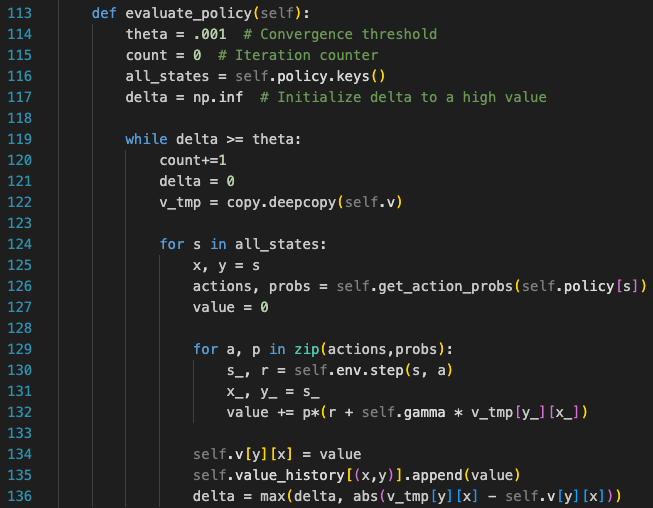
\includegraphics[width=0.8\textwidth]{images/policy_eval_impl.png}
    \caption{Policy Evaluation Implementation}
    \label{pe_impl}
\end{figure}

\noindent The implementation of the policy evaluation in Figure ~\ref{pe_impl} step involves computing the utility of each state while following a fixed policy. Similar to Value Iteration, we maintain two copies of the value map to track convergence, ensuring that updates in each iteration are based on the previous values. Convergence is determined when the maximum difference between the old and new state values satisfies $\Delta \leq \theta$, where $\theta$ is a small threshold.\vspace{10pt}

\noindent The core of the algorithm lies in lines 124 to 134, where the utility of each state is iteratively updated. Unlike Value Iteration, which evaluates all possible actions and selects the one maximizing expected utility, Policy Evaluation strictly follows the action prescribed by the current policy. This ensures that the value function stabilizes before proceeding to policy improvement.\vspace{10pt}

\noindent Throughout the evaluation process, the implementation allows flexibility in recording utility values, either at each iteration or only upon convergence.

\subsubsection{Policy Improvement}

\begin{figure}[H]
    \centering
    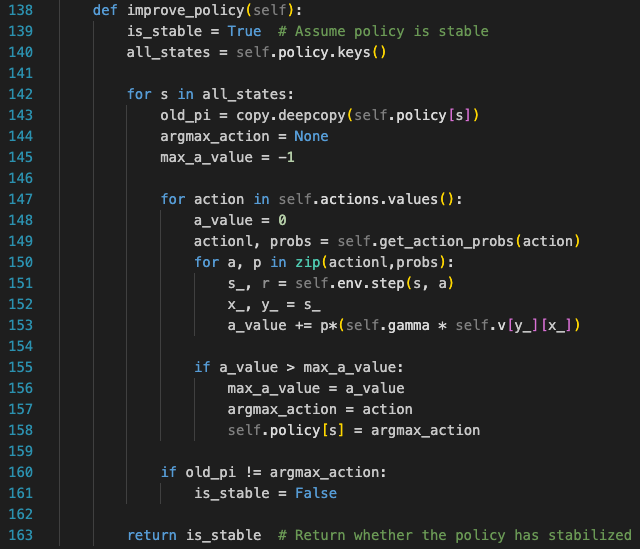
\includegraphics[width=0.8\textwidth]{images/policy_impr_impl.png}
    \caption{Policy Improvement Implementation}
    \label{pi_impl}
\end{figure}

\noindent In the Policy Improvement step, the policy is updated by selecting the action that maximizes the expected return based on the current value function. This process is implemented in lines 147 to 158 in Figure~\ref{pi_impl}, where the optimal action is chosen for each state (line 142). If the policy remains unchanged during this step, it is deemed optimal, and the algorithm terminates. Otherwise, the updated policy undergoes another iteration of evaluation and improvement until convergence. This is finalized in lines 160-161, where the algorithm checks whether the policy remains consistent across all states. If no further changes occur, the policy is considered stable, signifying convergence.

\begin{figure}[H]
    \centering
    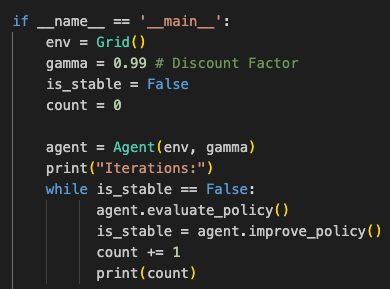
\includegraphics[width=0.8\textwidth]{images/policy_iter_impl.png}
    \caption{Policy Iteration Implementation}
    \label{pit_impl}
\end{figure}

\noindent Finally, the Policy Iteration algorithm, as shown in Figure~\ref{pit_impl}, integrates both the Policy Evaluation and Policy Improvement steps. The process iterates between evaluating the current policy and refining it until convergence is achieved, ensuring the policy remains optimal.

\subsection{Plot of Optimal Policy}
\begin{figure}[H]
    \centering
    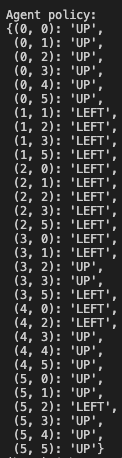
\includegraphics[width=0.2\textwidth]{images/pi_policy.png}
    \caption{Console Output of Policy Iteration}
    \label{pit_plot_policy}
\end{figure}

\begin{figure}[H]
    \centering
    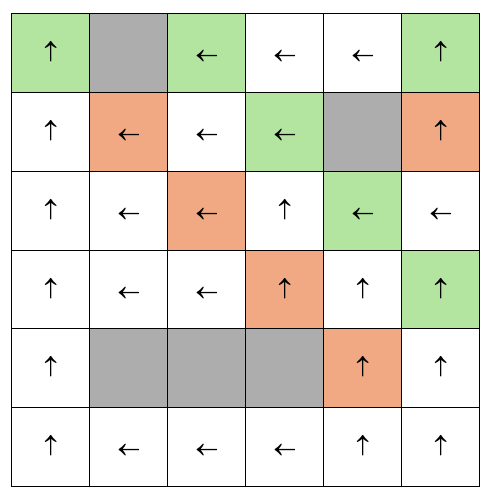
\includegraphics[width=0.6\textwidth]{images/vi_plot_policy.png}
    \caption{Plot of Optimal Policy}
    \label{pit_plot_policy_console}
\end{figure}

\noindent The final optimal policy shown in Figure ~\ref{pit_plot_policy} is identical to the one obtained from Value Iteration in Figure ~\ref{fig:vi_plot_policy}. The console output is shown in Figure ~\ref{pit_plot_policy_console}.

\subsection{Utility of All States}
\begin{figure}[H]
    \centering
    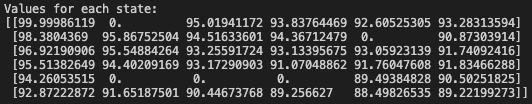
\includegraphics[width=0.8\textwidth]{images/pi_utility.png}
    \caption{Console Output of Value Iteration Utilities}
    \label{fig:pi_console_utility}
\end{figure}

\begin{figure}[H]
    \centering
    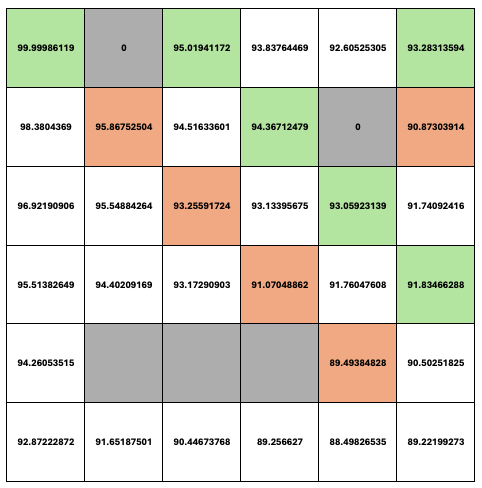
\includegraphics[width=1.0\textwidth]{images/pi_plot_utility.png}
    \caption{Plot of Utilities of All States}
    \label{fig:pi_plot_utility}
\end{figure}

Similar to Value Iteration, the upper limit of our utilities are bounded by the estimation of 100.

\subsection{Plot of Utility Estimates as a Function of the Number of Iterations}

\begin{figure}[H]
    \centering
    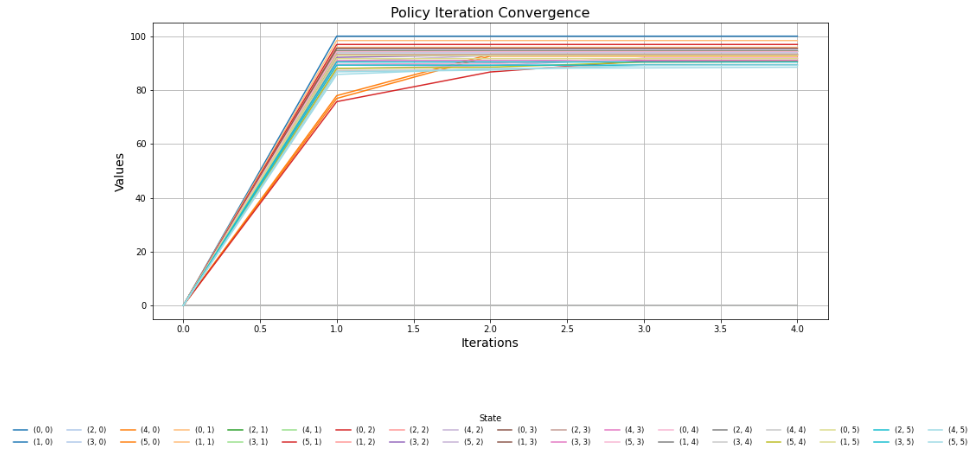
\includegraphics[width=1.0\textwidth, height=0.3\textheight]{images/pi_iteration.png}
    \caption{Plot of Utility Estimates \textbf{after} Policy Evaluation Convergence as a Function of the Number of Iterations}
    \label{fig:pi_plot_utility_iteration}
\end{figure}

\begin{figure}[H]
    \centering
    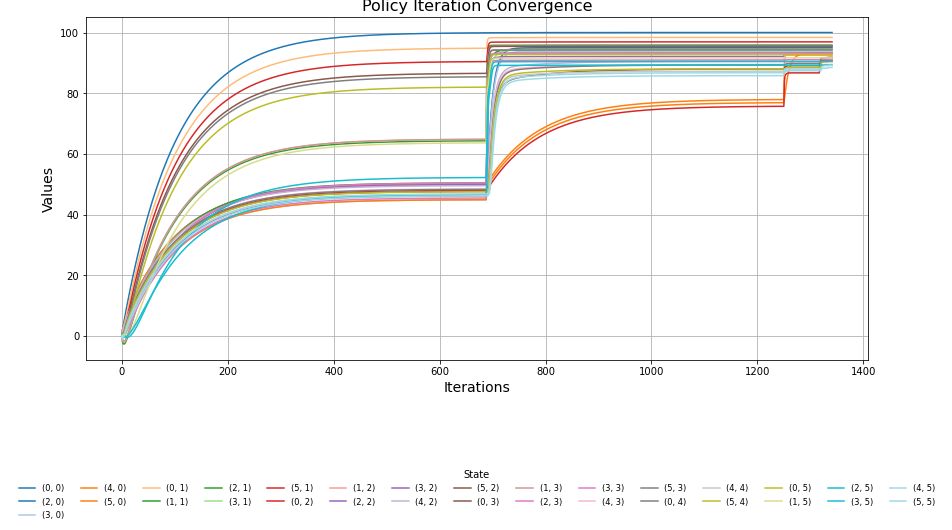
\includegraphics[width=1.0\textwidth]{images/pi_each_step.png}
    \caption{Plot of Utility Estimates \textbf{at each step} of Policy Evaluation Convergence as a Function of the Number of Iterations}
    \label{fig:pi_plot_utility_each_step}
\end{figure}

\noindent Similar to Value Iteration, $\theta = 0.001$. We observe that a total of 5 policy iterations is required to reach convergence, which is significantly lower than that of Value Iteration. However, the number of Policy Evaluation steps required is 1341. \vspace{10pt}

\noindent In Figure~\ref{fig:pi_plot_utility_iteration}, we observe that the utility estimates gradually converge as the number of iterations increases, eventually reaching a plateau when further updates no longer yield significant changes. This behavior aligns with the theoretical expectation that Policy Iteration will eventually arrive at an optimal policy. Additionally, the points at which the Policy Improvement step occurs can be identified by sharp changes in the gradient of the plotted lines. This trend is even more evident in Figure~\ref{fig:pi_plot_utility_each_step}, where distinct spikes in utility values correspond to policy updates. Within each Policy Evaluation phase, we see that the utility values under the current policy steadily increase before stabilizing, reflecting the iterative refinement of value estimates. These observations validate our understanding of the Policy Iteration algorithm, where alternating Policy Evaluation and Policy Improvement steps systematically refine the policy until convergence.